TODO: clean this up (lecture slides 27.10.22)

%%%%%%%%%%%%%%%%%%%%%%%%%%%%%%%%%%%%%%%%%%%%%%%%%
\chapter{Inter-process Communication (IPC)}
%%%%%%%%%%%%%%%%%%%%%%%%%%%%%%%%%%%%%%%%%%%%%%%%%

Inter-process communication means exchanging data between processes. There are different definitions. For example, the definition on Wikipedia says that \ac{IPC} is only the exchange of data between processes on one system i.e. of processes with access to shared memory. However, in this course, the definition is broader and includes the exchange of data between processes in a distributed system. \ac{IPC} is classified into three groups, which will be explained in detail in the following. Shared Memory, however, is less relevant for this course and will only be discussed briefly.

%%%%%%%%%%%%%%%%%%%%%%%%%%%%%%%%%%%%%%%%%%%%%%%%%
\section{Shared Memory}
%%%%%%%%%%%%%%%%%%%%%%%%%%%%%%%%%%%%%%%%%%%%%%%%%

\ac{IPC} using shared memory is less relevant for this course and will therefore only be discussed briefly.

When the processes have access to shared memory, they can communicate by writing and reading from that memory. This is often used in multithreaded applications, such as in \ac{OS} development or \ac{MPP} but is difficult to achieve in distributed systems. The communication is therefore implicit (i.e. there is no dedicated operation for sending messages). To synchronize processes and avoid race conditions, mutex locks or semaphores are used.


%%%%%%%%%%%%%%%%%%%%%%%%%%%%%%%%%%%%%%%%%%%%%%%%%
\section{Message Passing}
%%%%%%%%%%%%%%%%%%%%%%%%%%%%%%%%%%%%%%%%%%%%%%%%%

Message Passing is an explicit communication through dedicated send and receive operations.
Here, the synchronization between processes happens through blocking send or receive operations.

%------------------------------------------------
\subsection{Sockets}
%------------------------------------------------

Sockets define communication endpoints for processes through a socket address, which consists of the IP address and a port number. Different well-known port numbers are used for specific services e.g. HTTP servers listen on port 80 and ssh agents on port 22. In practice, there are two types of sockets for the two main transport layer protocols \textendash{} \ac{UDP} and \ac{TCP}. The corresponding sockets, therefore, provide the functionality, which is provided by the respective transport layer protocol.

Usually, many processes can send messages to the same endpoint of another process (e.g. many clients send messages to the same server socket address). In order to be able to respond to all processes separately, usually servers keep one socket for incoming requests and then open another socket for responding, such that there are $n+1$ sockets, given the number of clients is equal to $n$.




\subsubsection{User Datagram Protocol (UDP)}

Characteristics of communication via UDP sockets are the following:

\begin{itemize}
    \item Connection-less communication
    \item Messages are sent without acknowledgment, retries, ordering, congestion control and flow control.
    \item Message size is limited to 65 MB
    \item Very performant, because of limited comfort features and connection-less design.
    \item Sends are non-blocking
    \item If messages are sent before receiving socket is bound to this address, the messages are discarded at the destination machine
    \item Datagram header and payload are protected by a checksum, which ensures only valid messages are received. However, messages will not be corrected based on that, but rather be discarded.
    \item Usage examples: DNS, Voice over IP, Sensor Data, Video Streaming
\end{itemize}

Usually, usage of UPD-sockets follows the following scheme for the \textbf{sender}:

\begin{enumerate}
    \item Create a socket
    \item Send something over the socket to a destination socket address
    \item Close socket
\end{enumerate}

The workflow for the \textbf{receiving} side of a UPD-socket communication is usually the following:

\begin{enumerate}
    \item Bind a socket to the local server address
    \item Receive a message from the socket
    \item Close socket
\end{enumerate}


\subsubsection{Transmission Control Protocol (TCP)}

Characteristics for communication over TCP-sockets are the following:

\begin{itemize}
    \item Connection-oriented communication
    \item The message size is arbitrary but will be delivered as a byte stream. Therefore, a data format on top must ensure that the end of messages can be identified.
    \item Reliability: validity and integrity ensured by using checksums and retransmission.
    \item Flow control: Fast writer is blocked until a \textit{slow receiver} is ready for new bytes.
    \item Congestion control: Fast writer will slow down for \textit{slow networks}.
    \item Example Applications protocols: HTTP, FTP, SMTP
\end{itemize}

The TCP-socket interfaces on POSIX and Windows systems follow the so-called Barkley socket interface, which is shown in figure \ref{fig:barkley_socket_interface}.

\begin{figure}[h]
    \centering
    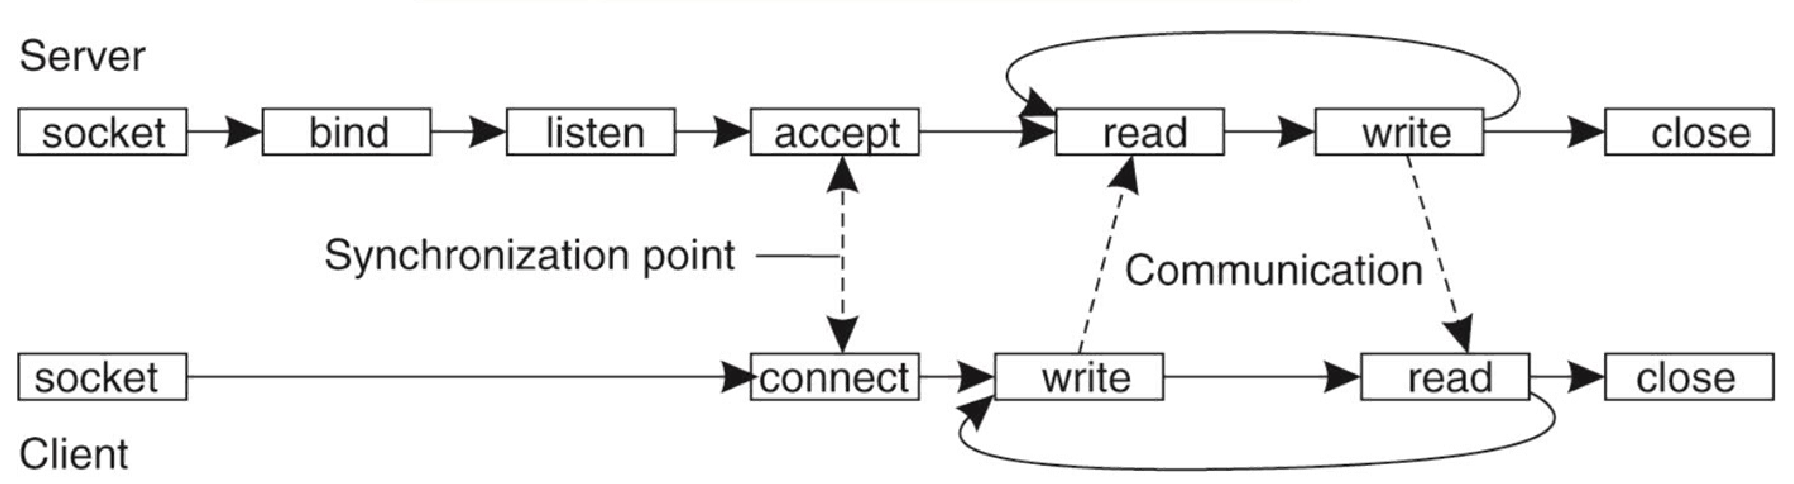
\includegraphics[width=\textwidth]{gfx/socket_lifecycle.png}
    \caption{Barkley Socket Interface}
    \label{fig:barkley_socket_interface}
\end{figure}

One challenge for TCP implementations is when to send messages in the local write buffer. One strategy would be to send them as soon as the buffer is full. But this is only useful when a large amount of data is written, otherwise, it would delay the send operations of small messages. Another approach, which was implemented in the past is to combine the previous approach with a timeout (e.g. 0.5 seconds), after which the buffer is guaranteed to be flushed. Nowadays, Nagle's algorithm is used. This flushes the buffer if it is full or if all of the previously sent packages have already been acknowledged.


%------------------------------------------------
\subsection{Transport Layer Alternatives}
%------------------------------------------------

TCP is by far the most used transport protocol for applications, which requires reliability. At the same time, it is old and not optimal. Therefore, there are other more modern transport protocols, which, however, are yet to be widely accepted.

The \ac{SCTP} offers message-oriented semantics (like TCP) but otherwise behaves like TCP to ensure reliability and its other useful features. Furthermore, reliability, ordering and fragemenütation of messages can be toggled in order to provide a more flexible interface for different use cases. Moreover, multi-streaming (multiple independent data streams for one connection e.g. one stream for messages, one stream for videos) and multi-homing (endpoints can have multiple IP addresses for failover) are supported.

The \ac{DCCP} provides fast and unreliable transmission of messages (like UDP) with additional congestion control. This protocol has not been accepted by the community and will probably die out.

\ac{QUIC} is a protocol designed by Google and is currently in the standardization process. It is implemented in Chrome, Chromium and other Google Apps. It intertwines with security (TSL) and application layer (HTTP) in order to increase its performance. This, however, violates the principle of distribution of concerns.


%------------------------------------------------
\subsection{Distributed Programming Languages}
%------------------------------------------------

Although distributed programming is of high interest, distributed programming languages have not been established yet. The reason is, that programmers do not like to learn new languages, especially if these are not widespread yet. Furthermore, one distributed programming language typically only supports one programming paradigm (OOP, functional programming ...), such that one distributed programming language can not make everybody happy. Moreover, the comfort of distributed programming languages can also partly be achieved through middleware. Nevertheless, research in this area is being done. Some examples of distributed programming languages are CSP, ARGUS, Linda, Emerald, Erlang and SCALA.

%%%%%%%%%%%%%%%%%%%%%%%%%%%%%%%%%%%%%%%%%%%%%%%%%
\section{Message Queues}
%%%%%%%%%%%%%%%%%%%%%%%%%%%%%%%%%%%%%%%%%%%%%%%%%



% \ac{IPC} can be split into three types, which will be explained in more detail in the following.

% \section{Shared Memory}

% NOTES:
% Implicit communication about shared memory.
% Synchronization using locks
% Widespread in OS and MPP
% DIfficult in DistSystems, where no shared memory exists -> emulate it if required

% Less relevant for this lecture

% \section{Message Passing}

% - Explicit communication through messages
% - synchronization through blocking receive and send operations
% - exactly what happens in distSyst, because we send messages over the transport layer

% TCP Sockets usage:
% connection cycle: (insert a picture from slide 15)
% Server: socket (creates port association for accepting multiple remote connections) -> bind -> listen -> accept -> read/write -> close
% Client: socket(create port association) -> connect -> write/read -> close
% - stream semantics
% - Server has many incoming connections on the same port. Therefore it must distinguish between the incoming connections. Therefore, one listener socket is used and then another transmission socket is created for each connected client. This way we then can read and write from different distinct sockets and also close them independently. This is somewhat a dirty pattern, however, it is the currently used pattern.

% UDP socket usage:
% Server: create socket -> loop{receive} -> close
% Client: create socket -> send to address+port -> end or send new message.
% - no connection
% - integrity: somehow yes. UDP will throw errors based on checksum, but not correct the error or resubmit the message
% - validity not provided
% - -> reliability not provided
% - UPD is the basis for sophisticated transport protocols, which might be better than TCP for some use cases.
% - message semantics, not stream semantics

% ### Other transport layers than UPD and TCP of today's age:
% - TCP is still by far the most common one
% - e.g. QUIC is another very fast transport layer protocol
% - IEFT Working Group TAPS works on a generic interface to transport layer. Such that programmers can use any transport protocol without changing their program code (accept maybe one variable determining the protocol)


% #### SCTP (slide 25)
% #### DCCP (slide 26)
% - separate header and data checksum -> if only data checksum is corrupted. Therefore, we can error handle it depending on the intact header. Otherwise (like in TCP) we must just throw corrupted packets away because e.g. the sequence number might not be correct.
% #### QUIC
% - implemented in chrome, chromium and some other apps
% - Contrary to other proposed protocols, this sees more acceptance due to Google's big influence.
% - less overhead on connection establishment (fewer handshake messages)
% - Is faster, because linking directly into TSL
% - Intertwines with HTTP2
% - On the contrary, if TSL or HTTP should be replaced, QUIC breaks, because it breaks the rules of layer separation.



% \section{Message Queues}

% \section{Distributed Programming Languages}

% - not accepted in the past, maybe coming up in the future
% - \ac{DRTS}